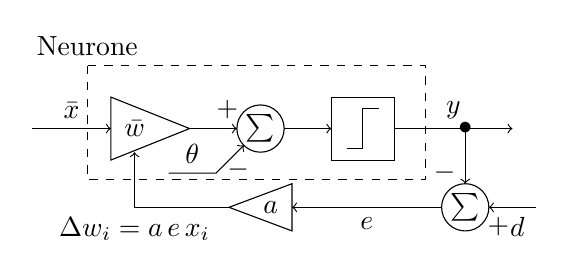
\begin{tikzpicture}
%
%% Ingresso
  \draw[->](0,0)--(1,0)
    node[pos=.5,above]{\(\bar{x}\)};
%
%% Cornice del neurone
  \draw [dashed, line join=round] (.7,.8) rectangle (5,-.65)
    node [pos=0, above] {Neurone};
%
%% Blocchi del neurone
  \draw (1,-.4)--(2,0)--(1,.4)--cycle;
  \node (w) at (1.3,0) {\(\bar{w}\)};
  \draw[->](2,0)-- ++(.6,0)
    node[pos=.8,above]{\(+\)};
  \draw[<-](2.9,0) ++(-135:.3)--
    ++(-135:.5) node[pos=.2,below]{$-$}
    -- ++(-.6,0)
    node[pos=.5,above]{$\theta$};
  \draw	(2.9,0) node{\(\sum\)} circle (.3);
  \draw[->](3.2,0)-- ++(.6,0);
  \draw (3.8,.4) rectangle ++(.8,-.8);
  \draw (4,-.25)-|(4.2,0)|-(4.4,.25);
%
%% Uscita
  \draw[->](4.6,0)-- ++(1.5,0)
    node[pos=.5,above]{\(y\)};
%
%% Retroazione
  \draw[->](5.5,0)-- ++(0,-.7)
    node[pos=0]{\(\bullet\)}
    node[pos=.8,left]{$-$};
  \draw	(5.5,-1) node{$\sum$} circle (.3);
  \draw[<-](5.8,-1)-- ++(.6,0)
    node[pos=0.2,below]{$+$}
    node[pos=0.6,below]{$d$};
  \draw[<-](1.3,-.3) |- (2.5,-1)
    node[pos=.5,,below]{\(\Delta w_i = a\,e\,x_i\)};
  \draw (3.3,-.7)--(2.5,-1)--(3.3,-1.3)--cycle;
  \node (a) at (3.03,-1) {$a$};
  \draw[<-](3.3,-1)--(5.2,-1)
    node[pos=.5,below]{$e$};
    
\end{tikzpicture}
